%! Author = mariuszindel
%! Date = 02.11.20

\section{Iteratoren}

\subsection{foreach-Loop}
\subsubsection{Übersicht}
\begin{itemize}
    \item Wird für das Iterieren über Collections verwendet
    \item Jumps
    \begin{itemize}
        \item continue $\rightarrow$ unterbricht aktuelle Iteration
        \item break $\rightarrow$ unterbricht gesammten Loop
    \end{itemize}
\end{itemize}
\subsubsection{Syntax}
Kriterien für «collection»:
\begin{itemize}
    \item Muss IEnumerable / IEnumerable<T> implementieren
    \item Muss einer Implementation von IEnumerable / IEnumerable<T> «ähneln»
    \begin{itemize}
        \item «collection» hat Methode GetEnumerator() mit Rückgabewert «e»
        \item «e» hat eine Methode MoveNext() mit Rückgabewert «bool»
        \item «e» hat ein Property «Current»
    \end{itemize}
\end{itemize}
\begin{lstlisting}
int[] list = new int[] { 1, 2, 3, 4, 5, 6 };
foreach (int i in list) {
    if (i == 3) continue;
    if (i == 5) break;
    Console.WriteLine(i);
}
\end{lstlisting}

\subsubsection{Sequenzdiagramm}
\begin{center}
    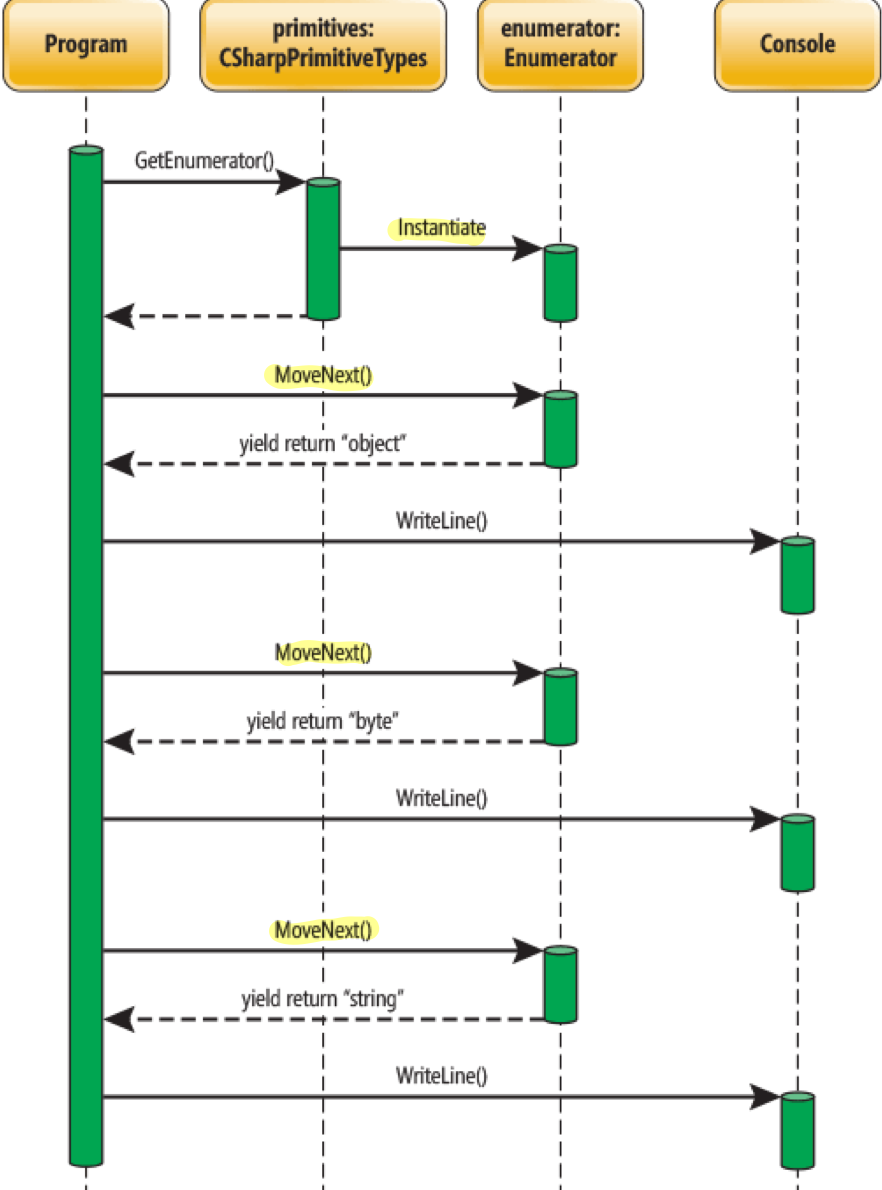
\includegraphics[scale=.33]{graphic/iterator/Sequenzdiagramm.png}
\end{center}


\subsection{Iteratoren}
\subsubsection{Interfaces}
Iterator = Enumerator!

\begin{itemize}
    \item Interface IEnumerable
\end{itemize}
\begin{lstlisting}
public interface IEnumerable {
    IEnumerator GetEnumerator();
}
\end{lstlisting}

\begin{itemize}
    \item Interface IEnumerator
\end{itemize}
\begin{lstlisting}
public interface IEnumerator {
    object Current { get; }
    bool MoveNext();
    void Reset();
}
\end{lstlisting}

\begin{itemize}
    \item Interface IEnumerable<T>
\end{itemize}
\begin{lstlisting}
public interface IEnumerable<out T>
    : IEnumerable {
    IEnumerator<T> GetEnumerator();
}
\end{lstlisting}

\begin{itemize}
    \item Interface IEnumerator<T>
\end{itemize}
\begin{lstlisting}
public interface IEnumerator<out T>
    : IDisposable, IEnumerator {
    T Current { get; }
    // Weitere Members werden vererbt
}
\end{lstlisting}


\subsubsection{Zugriff}
\begin{itemize}
    \item Mehrere aktive Iteratoren zur gleichen Zeit erlaubt
    \item Enumerator-Objekt muss Zustand vollständig kapseln
    \item Collection darf während Iteration nicht verändert werden
\end{itemize}


\subsubsection{Implementationsbeispiel (nicht-generisch)}
\begin{itemize}
    \item Klasse «MyList» als IEnumerable
    \item Klasse «MyEnumerator» als IEnumerator
\end{itemize}
\begin{lstlisting}
class MyList : IEnumerable {
    public IEnumerator GetEnumerator()
        { return new MyEnumerator(); }

    class MyEnumerator : IEnumerator {
    {

        public object Current }
            { get { /* ... */ } }

        public bool MoveNext() { /* ... */ }
        public void Reset() { /* ... */ }
    }
}
\end{lstlisting}

\subsubsection{Implementationsbeispiel (generisch)}
\begin{itemize}
    \item Klasse «MyList» als IEnumerable<T>
    \item Klasse «MyEnumerator» als IEnumerator<T>
\end{itemize}
\begin{lstlisting}
class MyIntList : IEnumerable<int> {

    public IEnumerator<int> GetEnumerator()
        { return new MyIntEnumerator(); }

    IEnumerator IEnumerable.GetEnumerator()
        { return GetEnumerator(); }

    class MyIntEnumerator : IEnumerator<int> {

        public int Current
            { get { /* ... */ } }
        object IEnumerator.Current
            { get { /* ... */ } }

        public bool MoveNext() { /* ... */ }
        public void Reset() { /* ... */ }
        public void Dispose() { /* ... */ }
    }
}
\end{lstlisting}

\subsection{Iterator-Methoden}
\subsubsection{Syntax}
Beinhaltet mindestens ein «yield return» Statement!
\begin{itemize}
    \item Gibt den nächsten Wert für die nächste Iteration eines «foreach» Loops zurück
    \item Syntax:\\
    yield return «expr»;
    \item «yield break» Statement terminiert die Iteration

\end{itemize}
\subsubsection{Implementationsbeispiel}
\begin{lstlisting}
class MyIntList {
    public IEnumerator<int> GetEnumerator() {
        yield return 1;
        yield return 3;
        yield break;
        yield return 6;
    }}
\end{lstlisting}

\subsection{Spezifische Iteratoren}
\subsubsection{Standard Iterator-Methode}
Iterator:
\begin{lstlisting}
class MyIntList {
    private int[] data = new int[10];

    // Standard Iterator
    public IEnumerator<int> GetEnumerator() {
        for (int i = 0; i < data.Length; i++)
        yield return data[i];
}}
\end{lstlisting}

Anwendung:
\begin{lstlisting}
MyIntList list = new MyIntList();
foreach (int elem in list) {
/* ... */ }
\end{lstlisting}


\subsubsection{Spezifische Iterator-Methode}
Iterator:
\begin{lstlisting}
class MyIntList {
    private int[] data = new int[10];

    // Spezifische Iterator-Methode
    public IEnumerable<int> Range(int from, int to) {
        for (int i = from; i < to; i++)
        yield return data[i];
}}
\end{lstlisting}

Anwendung:
\begin{lstlisting}
MyIntList list = new MyIntList();
foreach (int elem in list.Range(2, 7)) {
/* ... */
}
\end{lstlisting}


\subsubsection{Spezifisches Iterator-Property}
Iterator:
\begin{lstlisting}
class MyIntList {
    private int[] data = new int[10];

    // Spezifisches Iterator-Property
    public IEnumerable<int> Reverse {
        get {
            for (int i = data.Length - 1; i >= 0; i--)
                yield return data[i];
}}}
\end{lstlisting}

Anwendung:
\begin{lstlisting}
MyIntList list = new MyIntList();
foreach (int elem in list.Reverse) {
/* ... */
}
\end{lstlisting}

\subsection{Erweiterungsmethoden}
\subsubsection{Übersicht}
\begin{itemize}
    \item Erlaubt das Erweitern bestehender Klassen
    \item Signatur der Klasse wird nicht verändert
    \item Aufruf sieht jedoch so aus, als wäre es eine Methode auf der Klasse
    \item Muss in statischer Klasse deklariert sein
    \item Muss «static» sein
    \item «this» Schlüsselwort voranstehend
\end{itemize}

\subsubsection{Regeln}
\begin{itemize}
    \item Kein Zugriff auf interne Members aus Extension Methode
    \item «ToStringSafe» ist nur sichtbar, wenn der Namespace von «ExtensionMethods» importiert wurde
    \item Bei Konflikt mit Methode auf der Zielklasse gewinnt immer die eigene Methode
    \item Erlaubt auf Klassen / Structs / Interfaces / Delegates / Enumeratoren / Arrays
\end{itemize}
\begin{lstlisting}
public static class ExtensionMethods {
    static string ToStringSafe(this object obj) {
        return obj == null ? string.Empty : obj.ToString();
    }
    public static void Test() {
        int myInt = 0;
        object myObj = new object(); // Objects not null
        myInt.ToString();
        myInt.ToStringSafe();
        myObj.ToString();
        myObj.ToStringSafe(); // Object is null
        myObj = null;
        myObj.ToString(); // Error
        myObj.ToStringSafe(); // Works
}}
\end{lstlisting}

\subsection{Deferred Evaluation}
\subsubsection{Übersicht}
\begin{itemize}
    \item Aufruf von GetEnumerator() oder von Range(…) führt Iterator-Methode noch NICHT aus
    \item Erst der Aufruf von IEnumerator<T>.MoveNext()
    \item $\rightarrow$ Dies passiert implizit im «foreach» Loop
\end{itemize}
\subsubsection{Beispiel}

\subsubsection{Extension Methods und Iteratoren}
\begin{lstlisting}
public class Extensions
{
public static void ForeachIfGreaterThan11(IList<int> source, Action<int> action){
foreach (int elem in source)
{
    if (elem > 10) { action(elem); }
}}}

//neu zu:
public static class Extensions
{
    public static void ForeachIf<T>(
        this IEnumerable<T> source,
        Action<T> action,
        Predicate<T> predicate)
    {
        foreach (T elem in source)
        {
            if (predicate(elem)) {
                action(elem);
        } } }}
\end{lstlisting}

\subsubsection{Grafisch}
\begin{center}
    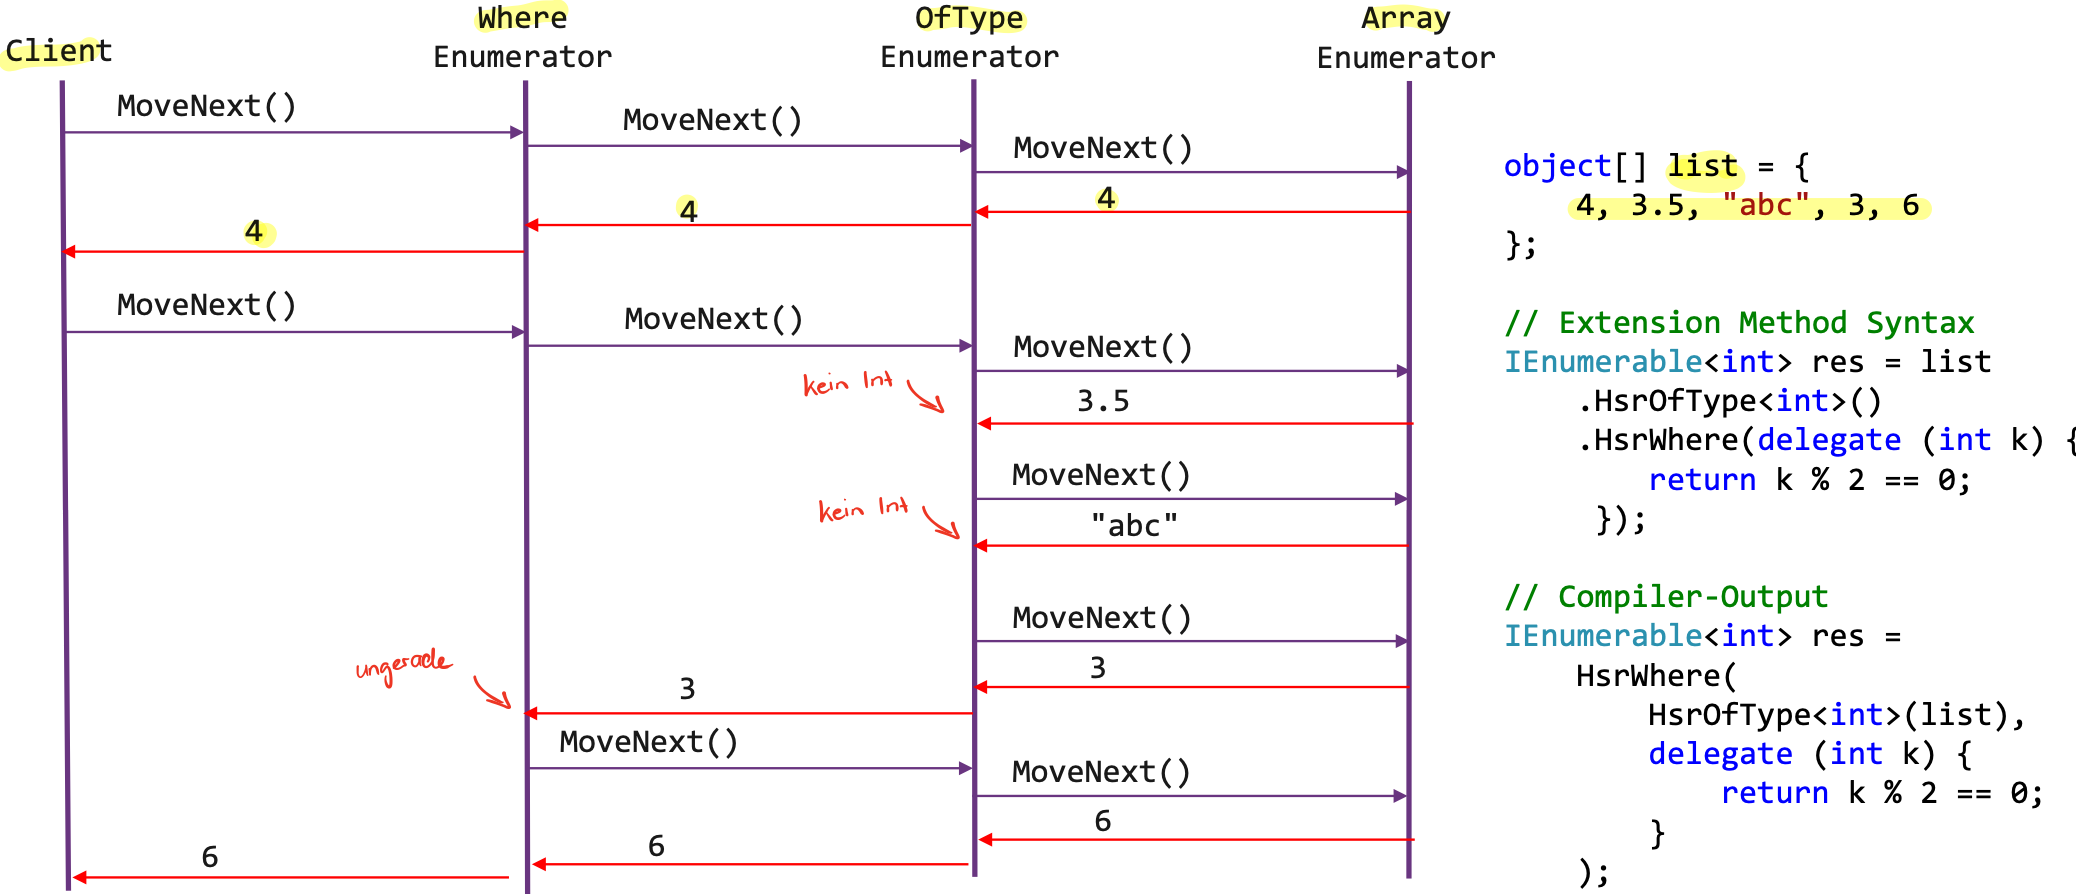
\includegraphics[scale=.24]{graphic/iterator/Deferred Evaluation.png}
\end{center}


\newpage

